\documentclass[twoside,b5paper,10pt]{article}
\usepackage{AUTstyle}

\usepackage{lipsum}                     % Dummytext
\usepackage{xargs}                      % Use more than one optional parameter in a new commands
\usepackage[pdftex,dvipsnames]{xcolor}  % Coloured text etc.

\usepackage[colorinlistoftodos,prependcaption,textsize=tiny]{todonotes}
\newcommandx{\unsure}[2][1=]{\todo[linecolor=red,backgroundcolor=red!25,bordercolor=red,#1]{#2}}
\newcommandx{\change}[2][1=]{\todo[linecolor=blue,backgroundcolor=blue!25,bordercolor=blue,#1]{#2}}
\newcommandx{\info}[2][1=]{\todo[linecolor=OliveGreen,backgroundcolor=OliveGreen!25,bordercolor=OliveGreen,#1]{#2}}
\newcommandx{\improvement}[2][1=]{\todo[linecolor=Plum,backgroundcolor=Plum!25,bordercolor=Plum,#1]{#2}}
\newcommandx{\thiswillnotshow}[2][1=]{\todo[disable,#1]{#2}}
\usepackage{tikz}
\usetikzlibrary{positioning}
\usepackage[siunitx, europeanresistors, americaninductors, voltage shift=0.5]{circuitikz}

\ctikzset{bipoles/thickness=1}
\ctikzset{bipoles/length=0.8cm}
\ctikzset{bipoles/diode/height=.375}
\ctikzset{bipoles/diode/width=.3}
\ctikzset{tripoles/thyristor/height=.8}
\ctikzset{tripoles/thyristor/width=1}
\ctikzset{bipoles/vsourceam/height/.initial=.7}
\ctikzset{bipoles/vsourceam/width/.initial=.7}
\tikzstyle{every node}=[font=\small]
\tikzstyle{every path}=[line width=0.8pt,line cap=round,line join=round]

\title{PMSM Motor Model for P-HIL Application}
\author{Dávid Kiss}

\institution{Department of Automation and Applied Informatics \\
Budapest University of Technology and Economics}

\email{david.kiss@aut.bme.hu}

\headerTitle{PMSM Motor Model for P-HIL Application \dots}
\headerAuthor{Dávid Kiss}


\begin{document}
\makeAutStyleTitle

\begin{abstract}
Electrical drive simulation is one of the key areas of the emerging trends in power electronics. There are many off-the-shelf solutions available on the market, even engineering tools, like MATLAB/Simulink developed it's own solution for the problem in the Simscape Electrical toolbox. These Solutions however are not open for modification, limiting the field in which they can be used. For motor simulation purposes, different approach seem to be necessary. Real-time execution also crucial in case of HIL\footnote{Hardware-in-the-Loop} and P-HIL\footnote{Power Hardware-in-the-Loop} application.
There are claims, the solutions from different suppliers are applicable for on-line simulation, aiming for HIL and P-HIL environments. This Paper introduces a custom developed motor model, usable for motor emulation and compares it with the PMSM model provided by MATLAB/Simulink.
\end{abstract}


\begin{keywords}
Simulation; PMSM; MATLAB; Real-Time AACS Workshop; (list of $5$-$7$ keywords in this
format)
\end{keywords}

\listoftodos

\section{Introduction}
\label{sec:Introdu}



\todo[inline]{Nincs még kész.}

\section{Mathematical model of a PMSM Machine}
\label{sec:matPMSM}

The Automotive industry always played a key role in innovation and always pioneered with new and emerging technologies. The situation is no different in the case of electrification nowadays. Electrical motors are the core element of modern hybrid (HEV) and Battery Electric Vehicle's (BEV) drivetrains. Volume and mass is a very limiting factor, especially in the case of BEV vehicles, because the saved mass and volume provides more space for the battery itself, providing higher range for the vehicle. Because of these reasons, 3-phase induction (IM\footnote{Induction Machine}) and PMSM\footnote{Permanent Magnet Synchronous Machine} machines are commonly used in traction (and other actuation) systems in the automotive industry. The difference between these two type of electrical machines is the source of the magnetic flux inside. In the case of the IM the magnetic field has to come from external excitation, in the PMSM machine, as the name suggests, the magnetic field is generated by the built-in permanent magnets. PMSM machines are especially superior in power density, however their drawback is the necessity of complex control algorithms and the expensive magnetic material.

\info[inline]{Itt még be kell hivatkozni Veszprémi könyvét meg írni arról, hogy miért király a PMSM!}


This paper details the mathematical description of the PMSM due to it's simplicity, with the following assumptions:
\begin{itemize}
  \item The machine is symmetrical ($L_d = L_q$)
  \item The stator winding are in star connection
  \item Losses are neglected (Ventilation, internal friction, iron losses)
  \item Coil inductance and resistances are constant
\end{itemize}

To derive the equations describing a PMSM machine, it worth to take a look on the external excitation DC machine, presented on Fig. \ref{fig:dc_machine}.

\begin{figure}[htb]
\begingroup
\tikzset{}
 \centerline{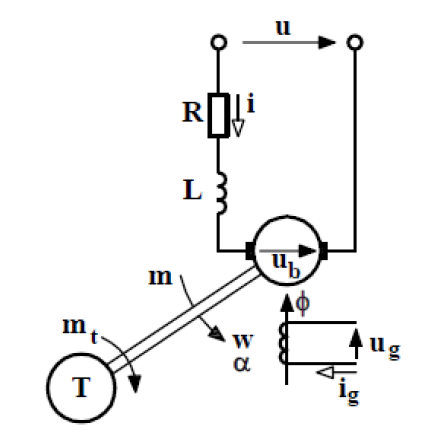
\includegraphics[width=.35\columnwidth]{.//Figure/dc_mot_veszpr.png}}
 \endgroup
 \caption{External excitation DC machine}
 \label{fig:dc_machine}
\end{figure}

From the equivalent circuit, Eq. \ref{eq:dc_dt} can be deducted. These Equations describing the relationship between the motor input voltage, current, torque and speed.


\begin{align} 
\label{eq:dc_dt}
u(t) &= i(t) + L\frac{di(t)}{dt} + u_b(t) \\ 
u_b(t) &= k\Phi{}\omega{}(t) \\
m(t) - m_t(t) &= \Theta{}\frac{d\omega{}(t)}{dt} \\
m(t) &= k\Phi{}i(t) \\
\omega{}(t) &= \frac{d\alpha(t)}{dt}
\end{align}


The electrical difference between the stator of a PMSM and a DC motor, the PMSM has a 3-phase winding with the spatial displacement of $\deg{120}$, connected in star. Each phase can modelled as a series RL and a voltage source. 

\begin{figure}[htb]
\begingroup
\tikzset{}
 \centerline{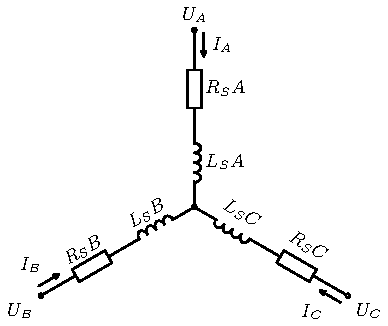
\includegraphics[width=.35\columnwidth]{.//Figure/threephase_winding.pdf}}
 \endgroup
 \caption{The equvalent circuit of a 3-phase motor winding}
 \label{fig:threephase_winding}
\end{figure}

If there no alternative current conducting path, other than the three phase connection (No parasitic coupling or short to earth), the 3-phase current system is symmetrical, meaning $I_A + I_B + I_C = 0$, thus the current phasor can be described with two independent values instead of three. To utilize this simplification, the Clark transformation is utilised, presented on Eq. \ref{eq:clark}

\begin{gather}
\label{eq:clark}
    \begin{bmatrix}
    \alpha \\ \beta \\ 0
    \end{bmatrix}
    =
    \frac{2}{3}
    \begin{bmatrix}
    1 & -\frac{1}{2} & -\frac{1}{2} \\[0.5em]
    0 & \frac{\sqrt{3}}{2} & -\frac{\sqrt{3}}{2} \\[0.5em]
    \frac{1}{2} & \frac{1}{2} & \frac{1}{2}
    \end{bmatrix}
    \begin{bmatrix}
    a \\ b \\ c
    \end{bmatrix}
\end{gather}

To get back the values in the original 3-phase reference frame, the Inverse-Clark transformation (Eq. \ref{eq:inv_clark}.) is used.

\begin{gather}
\label{eq:inv_clark}
    \begin{bmatrix}
     a \\ b \\ c
    \end{bmatrix}
    =
    \begin{bmatrix}
    1            & 0                  & 1             \\[0.5em]
    -\frac{1}{2} & \frac{\sqrt{3}}{2} & 1             \\[0.5em]
    -\frac{1}{2} & -\frac{\sqrt{3}}{2}& 1
    \end{bmatrix}
    \begin{bmatrix}
     \alpha \\ \beta \\ 0
    \end{bmatrix}
\end{gather}



\begin{gather}
\label{eq:park}
    \begin{bmatrix}
    d\\ q \\ 0
    \end{bmatrix}
    =
    \frac{2}{3}
    \begin{bmatrix}
    sin(\theta) & sin(\theta-\frac{2\pi}{3}) & sin(\theta+\frac{2\pi}{3}) \\[0.5em]
    cos(\theta) & cos(\theta-\frac{2\pi}{3}) & cos(\theta+\frac{2\pi}{3}) \\[0.5em]
    \frac{1}{2} & \frac{1}{2}                & \frac{1}{2}
    \end{bmatrix}
    \begin{bmatrix}
    a \\ b \\ c
    \end{bmatrix}
\end{gather}
\begin{gather}
\label{eq:inv_park}
    \begin{bmatrix}
    a \\ b \\ c
    \end{bmatrix}
    =
    \begin{bmatrix}
    sin(\theta)                & cos(\theta)                & 1                   \\[0.5em]
    sin(\theta-\frac{2\pi}{3}) & cos(\theta-\frac{2\pi}{3}) & 1                   \\[0.5em]
    sin(\theta+\frac{2\pi}{3}) & cos(\theta+\frac{2\pi}{3}) & 1
    \end{bmatrix}
    \begin{bmatrix}
    d\\ q \\ 0
    \end{bmatrix}
\end{gather}



\begin{align*} 
u(s) &= Ti(s) + Lsi(s) + u_b(s) \\ 
u_b(s) &= k\Phi{}\omega{}(s) \\
m(s) - m_t(s) &= \Theta{}s\omega{}(s) \\
m(s) &= k\Phi{}i(s) \\
\omega{}(t) &= s\alpha(s)
\end{align*}

 \begin{figure}[h]
        \centering
%%----start of first subfigure----
        \subfloat[Interior magnets]{
            \label{subfig:one} %% label for first subfigure
            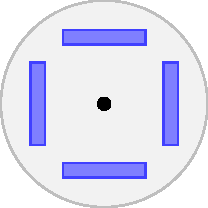
\includegraphics[width=0.2\linewidth]{Figure/motor_interior.pdf}}
        \hspace{0.02\linewidth}
%%----start of second subfigure----
        \subfloat[Surface mounted magnets]{
            \label{subfig:two} %% label for second subfigure
            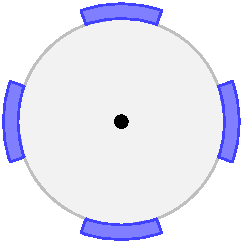
\includegraphics[width=0.2\linewidth]{Figure/motor_exterior.pdf}}
        \caption{PMSM Motor types}
        \label{fig:mot_sailient_non} %% label for entire figure
\end{figure}

 \begin{figure}[h]
        \centering
%%----start of first subfigure----
        \subfloat[Stator Reference frame]{
            \label{subfig:one} %% label for first subfigure
            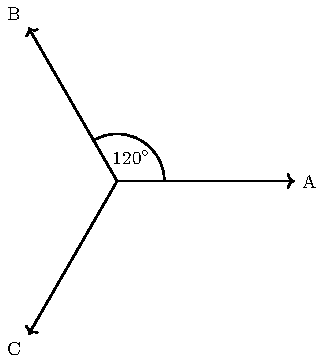
\includegraphics[width=0.3\linewidth]{Figure/coord_abc.pdf}}
        \hspace{0.02\linewidth}
%%----start of second subfigure----
        \subfloat[$\alpha\beta$ and $dq$ Reference frame]{
            \label{subfig:two} %% label for second subfigure
            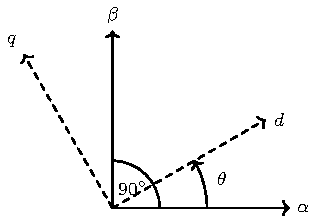
\includegraphics[width=0.3\linewidth]{Figure/coord_alpha_dq.pdf}}
        \caption{Different reference frames}
        \label{fig:bme} %% label for entire figure
\end{figure}


\begin{table}[htb]
\caption{Parameters of the example machine}
\begin{center}
\begin{tabular}{|r|c|c|}
\hline
\textbf{Parameter} & \textbf{Symbol} & \textbf{Value} \\
\hline
Nominal Power & $P_N$ & $90\ kW$ \\
\hline
Nominal RMS Voltage & $U_N$ & $400\ V$ \\
\hline
Nominal frequency & $f_N$ & $100\ Hz$ \\
\hline
Winding resistance & $R_s$ & $35.6\ m\Omega$ \\
\hline
Winding Inductance & $L\ =\ L_d\ =\ L_q$& $565.8\  \mu{}H$ \\
\hline
Motor Inertia & $\Theta$ & $0.0912\  kg\cdot{}m^2$ \\
\hline
Motor pole pairs & $pp$ & $1$ \\
\hline
Inverter Switching frequency & $f_{sw}$ & $5\ kHz$ \\
\hline

\end{tabular}
\end{center}
\label{tab:machine}
\end{table}

\section{Bibliography}
\label{sec:bib}

\section{The Simulink Built-In implementation}

\section{The custom implementation}

\section{Test Framework}

\section{Result of comarsion}


\section*{Acknowledgments}
 { \small The author would like to express his thanks to Dr. István Varjasi for his support as a scientific advisor.
This work has been supported by the Department of Automation and Applied Informatics}

\makeAutBib{reni,itemsetmining}

\end{document}
